% Options for packages loaded elsewhere
\PassOptionsToPackage{unicode}{hyperref}
\PassOptionsToPackage{hyphens}{url}
%
\documentclass[
]{book}
\usepackage{amsmath,amssymb}
\usepackage{lmodern}
\usepackage{ifxetex,ifluatex}
\ifnum 0\ifxetex 1\fi\ifluatex 1\fi=0 % if pdftex
  \usepackage[T1]{fontenc}
  \usepackage[utf8]{inputenc}
  \usepackage{textcomp} % provide euro and other symbols
\else % if luatex or xetex
  \usepackage{unicode-math}
  \defaultfontfeatures{Scale=MatchLowercase}
  \defaultfontfeatures[\rmfamily]{Ligatures=TeX,Scale=1}
\fi
% Use upquote if available, for straight quotes in verbatim environments
\IfFileExists{upquote.sty}{\usepackage{upquote}}{}
\IfFileExists{microtype.sty}{% use microtype if available
  \usepackage[]{microtype}
  \UseMicrotypeSet[protrusion]{basicmath} % disable protrusion for tt fonts
}{}
\makeatletter
\@ifundefined{KOMAClassName}{% if non-KOMA class
  \IfFileExists{parskip.sty}{%
    \usepackage{parskip}
  }{% else
    \setlength{\parindent}{0pt}
    \setlength{\parskip}{6pt plus 2pt minus 1pt}}
}{% if KOMA class
  \KOMAoptions{parskip=half}}
\makeatother
\usepackage{xcolor}
\IfFileExists{xurl.sty}{\usepackage{xurl}}{} % add URL line breaks if available
\IfFileExists{bookmark.sty}{\usepackage{bookmark}}{\usepackage{hyperref}}
\hypersetup{
  pdftitle={AMAT- Introducción a Ciencia de Datos y Machine Learning},
  pdfauthor={Karina Lizette Gamboa Puente; Oscar Arturo Bringas López},
  hidelinks,
  pdfcreator={LaTeX via pandoc}}
\urlstyle{same} % disable monospaced font for URLs
\usepackage{longtable,booktabs,array}
\usepackage{calc} % for calculating minipage widths
% Correct order of tables after \paragraph or \subparagraph
\usepackage{etoolbox}
\makeatletter
\patchcmd\longtable{\par}{\if@noskipsec\mbox{}\fi\par}{}{}
\makeatother
% Allow footnotes in longtable head/foot
\IfFileExists{footnotehyper.sty}{\usepackage{footnotehyper}}{\usepackage{footnote}}
\makesavenoteenv{longtable}
\usepackage{graphicx}
\makeatletter
\def\maxwidth{\ifdim\Gin@nat@width>\linewidth\linewidth\else\Gin@nat@width\fi}
\def\maxheight{\ifdim\Gin@nat@height>\textheight\textheight\else\Gin@nat@height\fi}
\makeatother
% Scale images if necessary, so that they will not overflow the page
% margins by default, and it is still possible to overwrite the defaults
% using explicit options in \includegraphics[width, height, ...]{}
\setkeys{Gin}{width=\maxwidth,height=\maxheight,keepaspectratio}
% Set default figure placement to htbp
\makeatletter
\def\fps@figure{htbp}
\makeatother
\setlength{\emergencystretch}{3em} % prevent overfull lines
\providecommand{\tightlist}{%
  \setlength{\itemsep}{0pt}\setlength{\parskip}{0pt}}
\setcounter{secnumdepth}{5}
\usepackage{booktabs}

\ifluatex
  \usepackage{selnolig}  % disable illegal ligatures
\fi
\usepackage[]{natbib}
\bibliographystyle{apalike}

\title{AMAT- Introducción a Ciencia de Datos y Machine Learning}
\author{Karina Lizette Gamboa Puente \and Oscar Arturo Bringas López}
\date{}

\begin{document}
\maketitle

{
\setcounter{tocdepth}{1}
\tableofcontents
}
\hypertarget{bienvenida}{%
\chapter{BIENVENIDA}\label{bienvenida}}

\hypertarget{objetivo}{%
\section{Objetivo}\label{objetivo}}

La primera parte del curso tiene como finalidad que el alumno tenga un entendimiento general de conceptos, técnicas, algoritmos y del proceso de desarrollo de proyectos de Ciencia de Datos.
Entenderá la diferencia entre Big Data, Machine Learning, Business Intelligence y Ciencia de Datos.
Todo lo anterior será cumplido mientras el alumno aprende las paqueterías y funciones más novedosas que se usan en R para Ciencia de Datos y las tecnologías que dan soporte a este software.

\textbf{Se asume que el alumno tiene conocimientos generales de estadística, bases matemáticas y de programación básica en R.}

\hypertarget{quienes-somos}{%
\section{¿Quienes somos?}\label{quienes-somos}}

\textbf{ACT. ARTURO BRINGAS}

\href{https://www.linkedin.com/in/arturo-bringas/}{LinkedIn}

Actuario, egresado de la Facultad de Ciencias y Maestría en Ciencia de Datos, ITAM.
Experiencia en el Departamento de Investigación Aplicada y Opinión de la UNAM diseñando metodologías estadísticas para estudios de percepción social. Es consultor de analítica predictiva para empresas y organizaciones como la Organización de las Naciones Unidas Contra la Droga y el Delito (UNODC), GNP, El Universal, Sinnia, Geek-end, entre otros. Actualmente se desempeña como consultor independiente participando en diferentes proyectos contribuyendo a empresas en temas de machine learning, estadística, series de tiempo, visualización de datos y análisis geoespacial. Adicionalmente, es profesor en el Diplomado de Metodologías de la Investigación Social impartido por la UNAM y profesor de machine learning y programación en R en AMAT

\begin{center}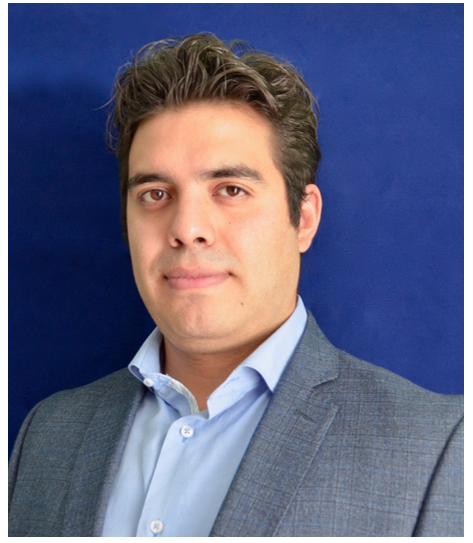
\includegraphics[width=6.57in]{img/arturo} \end{center}

\textbf{ACT. LIZETTE GAMBOA}

\href{https://www.linkedin.com/in/kalizzygam/}{LinkedIn}

Actuaria, egresada de la Facultad de Ciencias, UNAM, Maestría en Ciencia de Datos, ITAM.
Experiencia en áreas de analítica predictiva, e inteligencia del negocio, Lead Data Scientist en consultoría en diferentes proyectos con empresas de tecnología, retail y del sector asegurador y financiero. Experta en entendimiento de negocio para la correcta implementación de algoritmos de inteligencia y explotación de datos. Consultoras actuales: CLOSTER y RakenDataGroup. Experiencia en GNP, Activer Banco y Casa de Bolsa, PlayCity Casinos, entre otros.

\begin{center}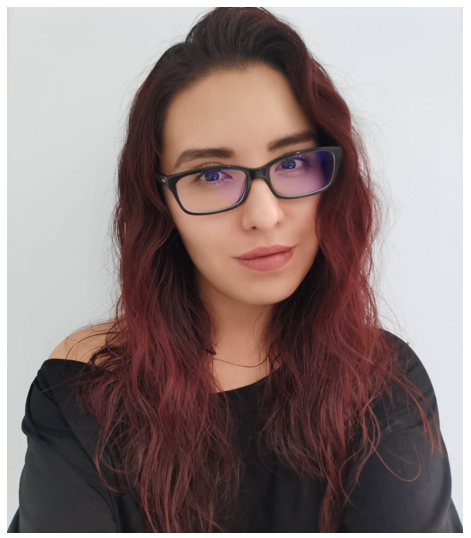
\includegraphics[width=6.54in]{img/lizzy} \end{center}

  \bibliography{book.bib,packages.bib}

\end{document}
